\newpage


%%%%%%%%%%%%%%%%%  Θ1
\begin{justify}
{\bf  Θ.1} (10) Για κάθε $T>0$ υπολογίστε το ολοκλήρωμα και σχεδιάστε
την συνάρτηση αυτοομοιότητας της συνάρτησης:
\end{justify}

\[
    \phi(t) =
\left\{
	\begin{array}{ll}
		\frac{1}{\sqrt{T}} &, \mbox{αν } |t| \leq \frac{T}{2} \\
		0 &, \mbox{διαφορετικά.}
	\end{array}
\right.
\]


\begin{justify}
\textbf{Λύση:}\\
H συνάρτηση αυτοομοιότητας της $\phi(t)$ ορίζεται ως $R_{\phi\phi}(\tau)=\int_{-\infty}^{+\infty} \phi(t+\tau)\phi(t)\,d\tau, \hspace{1.5em} \forall t \epsilon \mathbb{R}$.\\
Επιπλέον το $\phi(t+\tau)$:
    
\[
    \phi(t+\tau) =
\left\{
	\begin{array}{ll}
		\frac{1}{\sqrt{T}} &, \mbox{αν } |t+\tau| \leq \frac{T}{2} \\
		0 &, \mbox{διαφορετικά.}
	\end{array}
\right.
\]
\end{justify}

\begin{justify}
    
Παρατηρούμε ότι:
\newline
$\int_{-\infty}^{+\infty} \phi(t+\tau)\phi(t)\,d\tau, 
                                        \hspace{1.5em} t=s-\tau$
\newline
$\int_{-\infty}^{+\infty} \phi(s)\phi(s-\tau)\,ds, 
                                        \hspace{1.5em} s=\tau-u$
\newline
$\int_{-\infty}^{+\infty} \phi(\tau-u)\phi(-u)\,du, 
                                        \hspace{1.5em} \phi(-u)=g(u)$
                                        \newline
$\int_{-\infty}^{+\infty} \phi(\tau-u)g(u)\,du = \phi(\tau)*g(\tau)=\phi(\tau)*\phi(-\tau)$
\end{justify}

%%%%%%%%%Περιπτωση Θ1.1
\begin{justify}
Άρα με βάση την μεθοδολογία της συνέλιξης καταλήγουμε στις εξής περιπτώσεις:\newline\newline
{\bf 1\textsuperscript{η} Περίπτωση:}  $\tau+T<-\frac{T}{2}$
\[
R_{\phi\phi}(\tau)=0, \forall \tau \epsilon (-\infty,-T)      
\]
\end{justify}

%%%%%%%%%Περιπτωση Θ1.2
\begin{justify}
{\bf 2\textsuperscript{η} Περίπτωση:}  $\tau+\frac{T}{2}\geq -\frac{T}{2}$ και 
$\tau-\frac{T}{2}< -\frac{T}{2}$ 
\[
R_{\phi\phi}(\tau)=\int_{-\frac{T}{2}}^{\tau+\frac{T}{2}} \phi(t+\tau)\phi(t)\,d\tau =
\int_{-\frac{T}{2}}^{\tau+\frac{T}{2}} \frac{1}{\sqrt{T}}\frac{1}{\sqrt{T}}\,d\tau =
\frac{1}{T}[\tau]_{-\frac{T}{2}}^{\tau+\frac{T}{2}}
= \frac{1}{T}(\tau+\frac{T}{2}+\frac{T}{2})=1+\frac{\tau}{T} \hspace{1.5em} \forall\tau\epsilon[-T,0)\]
\end{justify}

%%%%%%%%%Περιπτωση Θ1.3
\begin{justify}
{\bf 3\textsuperscript{η} Περίπτωση:} $\tau-\frac{T}{2}\geq -\frac{T}{2}$ και 
$\tau-\frac{T}{2}< \frac{T}{2}$ 
\[
R_{\phi\phi}(\tau)=\int_{\tau-\frac{T}{2}}^{\frac{T}{2}} \frac{1}{T}\,d\tau = 
\frac{1}{T}[\tau]_{\tau-\frac{T}{2}}^{\frac{T}{2}} = \frac{1}{T}(\frac{T}{2}-\tau+\frac{T}{2})
=1-\frac{\tau}{T} \hspace{1.5em} \forall\tau\epsilon[0,T)
\]
\end{justify}

%%%%%%%%%Περιπτωση Θ1.4
\begin{justify}
{\bf 4\textsuperscript{η} Περίπτωση:}  $\tau-\frac{T}{2}\geq\frac{T}{2}$
\[
R_{\phi\phi}(\tau)=0, \forall \tau \epsilon [T,+\infty)      
\]
\end{justify}

\newpage

\begin{justify}
Οπότε:
\[
R_{\phi\phi}(\tau)= 
\left\{
	\begin{array}{lll}
		1+\frac{\tau}{T} &, \mbox{αν } -T \leq \tau < 0 \\
        1-\frac{\tau}{T} &, \mbox{αν } 0 \leq \tau < T \\
		0 &, \mbox{διαφορετικά.}
	\end{array}
\right.
\]
\end{justify}

%%%%%%PLOT
\begin{center}
    \centering
    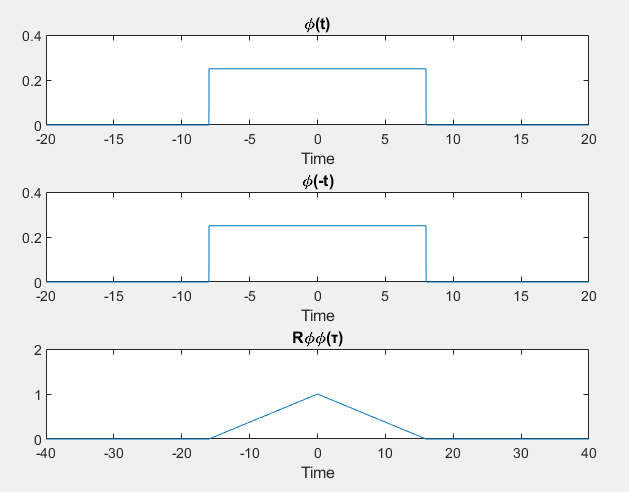
\includegraphics[width=0.8\textwidth]{THETA/Images/theta.fig1.png} % Adjust width as neededfilename of your images
    \label{fig:third_image}
\end{center}


%%%%%%%%%%%%%%%%%  Θ2
\begin{justify}
{\bf  Θ.2} (10) Επαναλάβετε την ίδια διαδικασία για $\phi(t-2)$.\\\\
\textbf{Λύση:}\\
Αρχικά θα υπολογίσουμε την $\phi(t-2)$:
\[
    \phi(t-2) =
\left\{
	\begin{array}{ll}
		\frac{1}{\sqrt{T}} &, \mbox{αν} -\frac{T}{2}+2 \leq t \leq \frac{T}{2} + 2 \\
		0 &, \mbox{διαφορετικά.}
	\end{array}
\right.
\]
\end{justify}

\begin{justify}
H συνάρτηση αυτοομοιότητας της $\phi(t)$ ορίζεται ως $R_{\phi\phi}=\int_{-\infty}^{+\infty} \phi(t-2+\tau)\phi(t-2)\,d\tau, \hspace{1.5em} \forall t \epsilon \mathbb{R}$.\newline
Βάση του {\bf Θ.1} προχωράμε στη συνέλιξη και καταλήγουμε στις εξής περιπτώσεις:
\end{justify}

%%%%%%%%%Περιπτωση Θ2.1
\begin{justify}
{\bf 1\textsuperscript{η} Περίπτωση:}  $\tau+\frac{T}{2}+2<-\frac{T}{2}$
\[
R_{\phi\phi}(\tau)=0, \forall \tau \epsilon (-\infty,-T)      
\]
\end{justify}

%%%%%%%%%Περιπτωση Θ2.2
\begin{justify}
{\bf 2\textsuperscript{η} Περίπτωση:}  $\tau+\frac{T}{2}+2\geq-\frac{T}{2}$ και $\tau-\frac{T}{2}+2<-\frac{T}{2} $
\[
R_{\phi\phi}(\tau)=\int_{-\frac{T}{2}+2}^{\tau+2+\frac{T}{2}} \frac{1}{T}\,d\tau = 
\frac{1}{T}[\tau]_{-\frac{T}{2}+2}^{\tau+2+\frac{T}{2}} = \frac{\tau+2+\frac{T}{2}+\frac{T}{2}-2}{T}
=1+\frac{\tau}{T} \hspace{1.5em} \forall\tau\epsilon[-T,0)
\]
\end{justify}

%%%%%%%%%Περιπτωση Θ2.3
\begin{justify}
{\bf 3\textsuperscript{η} Περίπτωση:}  $\tau-\frac{T}{2}+2\geq-\frac{T}{2}$ και $\tau-\frac{T}{2}+2<\frac{T}{2} $
\[
R_{\phi\phi}(\tau)=\int_{\tau-\frac{T}{2}+2}^{\frac{T}{2}+2} \frac{1}{T}\,d\tau = 
\frac{1}{T}[\tau]_{\tau-\frac{T}{2}+2}^{\frac{T}{2}+2} = \frac{\frac{T}{2}-\tau+\frac{T}{2}}{T}
=1-\frac{\tau}{T} \hspace{1.5em} \forall\tau\epsilon[0,T)
\]
\end{justify}

%%%%%%%%%Περιπτωση Θ2.4
\begin{justify}
{\bf 4\textsuperscript{η} Περίπτωση:}  $\tau-\frac{T}{2}+2\geq\frac{T}{2}$
\[
R_{\phi\phi}(\tau)=0, \forall \tau \epsilon [T,+\infty)      
\]
\end{justify}

\vspace{0.5cm}

\begin{justify}
Οπότε τελικά:
\[
R_{\phi\phi}(\tau)= 
\left\{
	\begin{array}{lll}
		1+\frac{\tau}{T} &, \mbox{αν } -T \leq \tau < 0 \\
        1-\frac{\tau}{T} &, \mbox{αν } 0 \leq \tau < T \\
		0 &, \mbox{διαφορετικά.}
	\end{array}
\right.
\]
\end{justify}

%%%%%%PLOT
\begin{center}
    \centering
    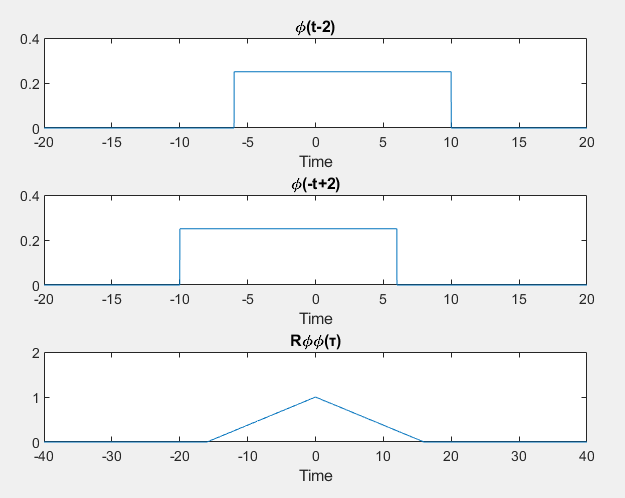
\includegraphics[width=0.8\textwidth]{THETA/Images/theta.fig2.png} % Adjust width as neededfilename of your images
    \label{fig:third_image}
\end{center}


\begin{justify}
Παρατηρούμε ότι οι συναρτήσεις αυτοομοιότητας των ερωτημάτων {\bf Θ.1} και {\bf Θ.2} είναι πανομοιότυπες. Λόγω αυτού βγαίνει το συμπέρασμα πως η $R_{\phi\phi}(\tau)$ δεν επηρεάζεται από τις χρονικές μετατοπίσεις της $\phi(t)$.
\end{justify}

\newpage


%%%%%%%%%%%%%%%%%  Θ3
\begin{justify}
{\bf  Θ.3} (10)Να επαναλάβετε για την:
\[
\phi(t)= 
\left\{
	\begin{array}{lll}
		\frac{1}{\sqrt{T}} &, \mbox{αν } 0 \leq t < \frac{T}{2} \\
        -\frac{1}{\sqrt{T}} &, \mbox{αν } \frac{T}{2} \leq t \leq T \\
		0 &, \mbox{διαφορετικά.}
	\end{array}
\right.
\]
\end{justify}

\begin{justify}
\textbf{Λύση:}\\
Θα κινηθούμε όμοια με το {\bf Θ.1} οπότε:
\[
\phi(t+\tau)= 
\left\{
	\begin{array}{lll}
		\frac{1}{\sqrt{T}} &, \mbox{αν } 0 \leq t+\tau < \frac{T}{2} \\
        -\frac{1}{\sqrt{T}} &, \mbox{αν } \frac{T}{2} \leq t+\tau \leq T \\
		0 &, \mbox{διαφορετικά.}
	\end{array}
\right.
\]
και καταλήγουμε στις εξής περιπτώσεις της συνέλιξης:
\end{justify}

%%%%%%%%%Περιπτωση Θ3.1
\begin{justify}
{\bf 1\textsuperscript{η} Περίπτωση:}  $\tau+T<0$
\[
R_{\phi\phi}(\tau)=0, \forall \tau \epsilon (-\infty,-T)      
\]
\end{justify}

%%%%%%%%%Περιπτωση Θ3.2
\begin{justify}
{\bf 2\textsuperscript{η} Περίπτωση:}  $\tau+T\geq0$ και $\tau+\frac{T}{2}<0$
\[
R_{\phi\phi}(\tau)=\int_{0}^{\tau+T} -\frac{1}{\sqrt{T}}\frac{1}{\sqrt{T}}\,d\tau =
\int_{0}^{\tau+T} -\frac{1}{T}\,d\tau=
-\frac{1}{T}[\tau]_{0}^{\tau+T} =\frac{-\tau-T}{T}
=-1-\frac{\tau}{T} \hspace{1.5em} \forall\tau\epsilon[-T,-\frac{T}{2})
\]
\end{justify}

%%%%%%%%%Περιπτωση Θ3.3
\begin{justify}
{\bf 3\textsuperscript{η} Περίπτωση:}  $\tau+\frac{T}{2}\geq0$ και $\tau<0$
\[
R_{\phi\phi}(\tau)=\int_{0}^{\tau+\frac{T}{2}}\frac{1}{T}\,d\tau+
\int_{\tau+\frac{T}{2}}^{\frac{T}{2}}-\frac{1}{T}\,d\tau+
\int_{\frac{T}{2}}^{\tau+T}\frac{1}{T}\,d\tau
=\frac{1}{T}([\tau]_{0}^{\tau+\frac{T}{2}}-[\tau]_{\tau+\frac{T}{2}}^{\frac{T}{2}}+
[\tau]_{\frac{T}{2}}^{\tau+T})
\]
\[
=\frac{1}{T}(\tau+\frac{T}{2}-\frac{T}{2}+\tau+\frac{T}{2}+\tau+T-\frac{T}{2})
=1+\frac{3\tau}{T}\hspace{1.5em} \forall\tau\epsilon[-\frac{T}{2},0)
\]
\end{justify}

%%%%%%%%%Περιπτωση Θ3.4
\begin{justify}
{\bf 4\textsuperscript{η} Περίπτωση:}  $\tau\geq0$ και $\tau<\frac{T}{2}$
\[
R_{\phi\phi}(\tau)=\int_{\tau}^{\frac{T}{2}}\frac{1}{T}\,d\tau+
\int_{\frac{T}{2}}^{\tau+\frac{T}{2}}-\frac{1}{T}\,d\tau+
\int_{\tau+\frac{T}{2}}^{T}\frac{1}{T}\,d\tau
=\frac{1}{T}([\tau]_{\tau}^{\frac{T}{2}}-[\tau]_{\frac{T}{2}}^{\tau+\frac{T}{2}}+
[\tau]_{\tau+\frac{T}{2}}^{T})
\]
\[
=\frac{1}{T}(\frac{T}{2}-\tau-\tau-\frac{T}{2}+\frac{T}{2}+T-\tau-\frac{T}{2})
=1-\frac{3\tau}{T}\hspace{1.5em} \forall\tau\epsilon[0,\frac{T}{2})
\]
\end{justify}

\newpage

%%%%%%%%%Περιπτωση Θ3.5
\begin{justify}
{\bf 5\textsuperscript{η} Περίπτωση:}  $\tau\geq\frac{T}{2}$ και $\tau\leq T$
\[
R_{\phi\phi}(\tau)=\int_{\tau}^{T} -\frac{1}{T}\,d\tau=
-\frac{1}{T}[\tau]_{\tau}^{T} =\frac{\tau-T}{T}
=-1+\frac{\tau}{T} \hspace{1.5em} \forall\tau\epsilon[\frac{T}{2},T]
\]
\end{justify}

%%%%%%%%%Περιπτωση Θ3.6
\begin{justify}
{\bf 6\textsuperscript{η} Περίπτωση:}  $\tau>T$
\[
R_{\phi\phi}(\tau)=0, \forall \tau \epsilon (T,\infty)      
\]
\end{justify}

\begin{justify}
Οπότε τελικά:
\[
R_{\phi\phi}(\tau)= 
\left\{
	\begin{array}{lllll}
		-1-\frac{\tau}{T} &, \mbox{αν } -T \leq \tau < -\frac{T}{2} \\
        1+\frac{3\tau}{T} &, \mbox{αν }  -\frac{T}{2} \leq \tau <0\\
        1-\frac{3\tau}{T} &, \mbox{αν } 0 \leq \tau <\frac{T}{2}\\
        -1+\frac{\tau}{T} &, \mbox{αν } \frac{T}{2} \leq \tau \leq T\\
		0 &, \mbox{διαφορετικά.}
	\end{array}
\right.
\]
\end{justify}

\vspace{1cm}

%%%%%%PLOT
\begin{center}
    \centering
    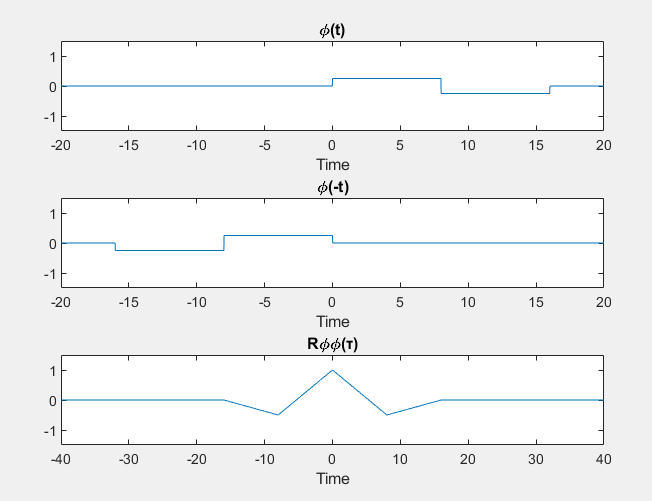
\includegraphics[width=0.8\textwidth]{THETA/Images/theta.fig3.png} % Adjust width as neededfilename of your images
    \label{fig:third_image}
\end{center}
